\chapter{Algorithm and Model Creation}

\section{Execution Environment}

Execution occurred in a real-time partially synchronous environment.
The execution environment was subject to omission failures.
Processes synchronized their clocks and executed steps of the election algorithm at predefined intervals.
Processes with clocks that were not sufficiently synchronized could not form groups.
For this work, process execution occurred in an environment where the clocks were sufficiently synchronized to consistently form groups.
In the real-time environment, messages that were delayed and missed their real-time deadlines had the same appearance as an omitted message.
The execution environment for the election algorithm had a omission fault occurrence modeled as a Bernoulli trial.
In this model, each message had some probability $p$ of being delivered within the timing constraints imposed by the real-time schedule.
For the purpose of analyzing the effects of omission failures, processes were not subject to other faults.

\section{Election Algorithm Overview}

A state machine for the election portion of the invitation-election algorithm is shown in Figure \ref{fig:statemachine}.
In the normal state, the election algorithm regularly searches for other coordinators to join with.
When another coordinator is identified the identifying coordinator will attempt to invite the other coordinator to their group.
In the invitation election algorithm, processes are assigned a priority based on their process ID.
The coordinator with the highest priority is the first to send invites.
After a brief delay, if it appears that coordinator did not send their invites, the next highest process will send their invites.
Coordinators that receive invites will forward the invite to its group members.
Processes that receive an invite that are not already in an election will accept the invite.
Once a timeout expires, the coordinator will send a ``Ready'' message with a list of peers to all processes that accepted the invite.
The invited processes have timeouts for when they expect the ready message to arrive.
If the message does not arrive in time, the process will enter the recovery state where it resets to a group by itself.

\begin{figure*}[!t]
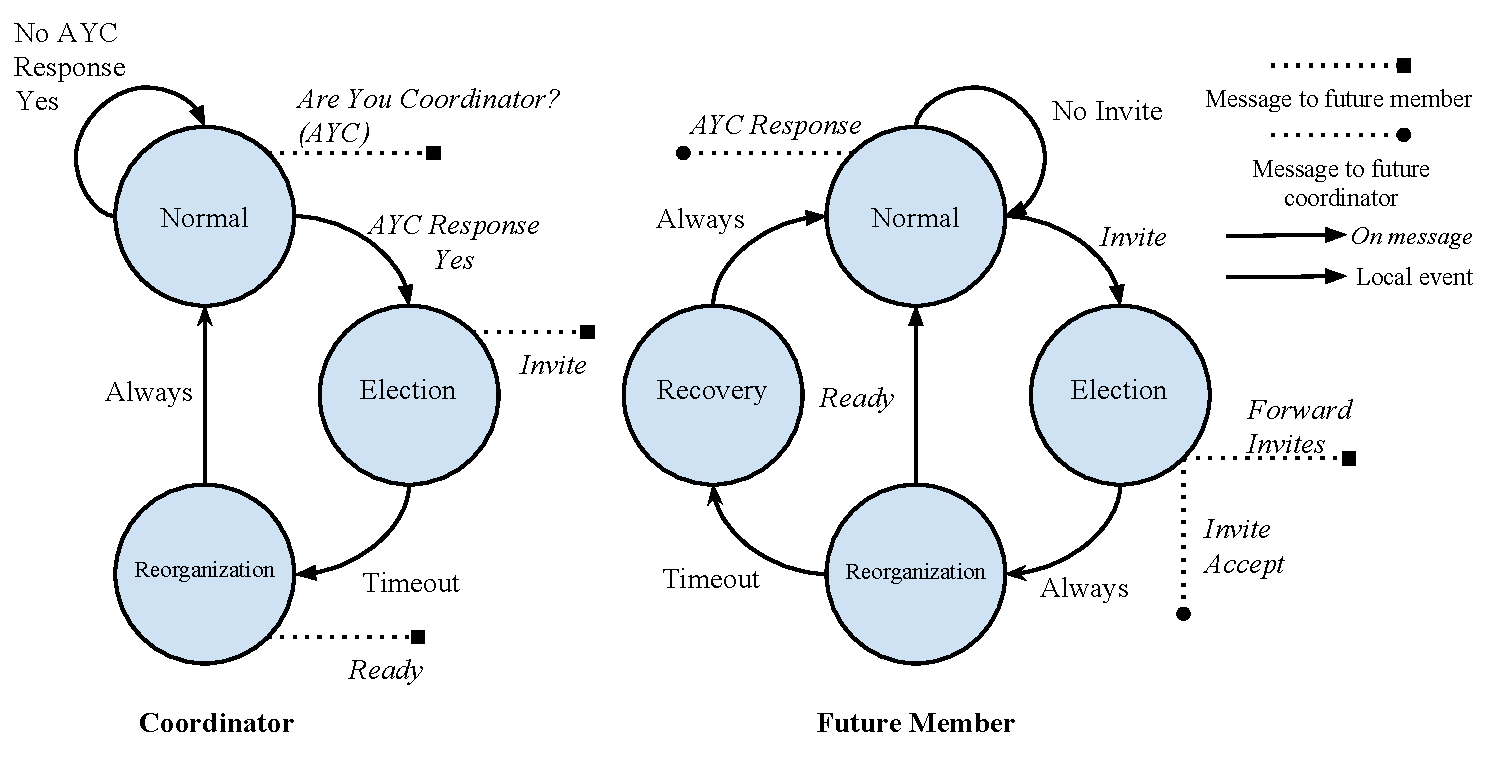
\includegraphics[width=\linewidth]{LeaderElectionStateDiagram.pdf}
\caption[State machine for an election]{State machine for an election. Processes start as coordinators in the ``Normal'' state and search for other coordinators to join with. Processes immediately respond to \ac{AYC} messages they receive. The algorithm was modified by adding a ``Ready Acknowledgment'' message as the final step of completing the election. Additionally, processes only accept invites if they have received an ``\ac{AYC} Response'' message from the inviting process.}
\label{fig:statemachine}
\end{figure*}

Once a group is formed it must be maintained.
To do this, processes occasionally exchange messages to verify the other is still reachable.
This interaction is shown in Figure \ref{fig:statemachine2}.
Coordinators send ``Are You Coordinator'' messages to members of its group to check if the process has left the group.
Group members send ``Are You There'' messages to the coordinator to verify they haven't been removed from the group, and to ensure the coordinator is still alive.
If processes fail to reply to received message before a timeout, they will leave the group.
Leaving the group can either be caused by the coordinator removing the process, or the process can enter a recovery state and leave the group, forming a new group by itself.

\begin{figure*}[!t]
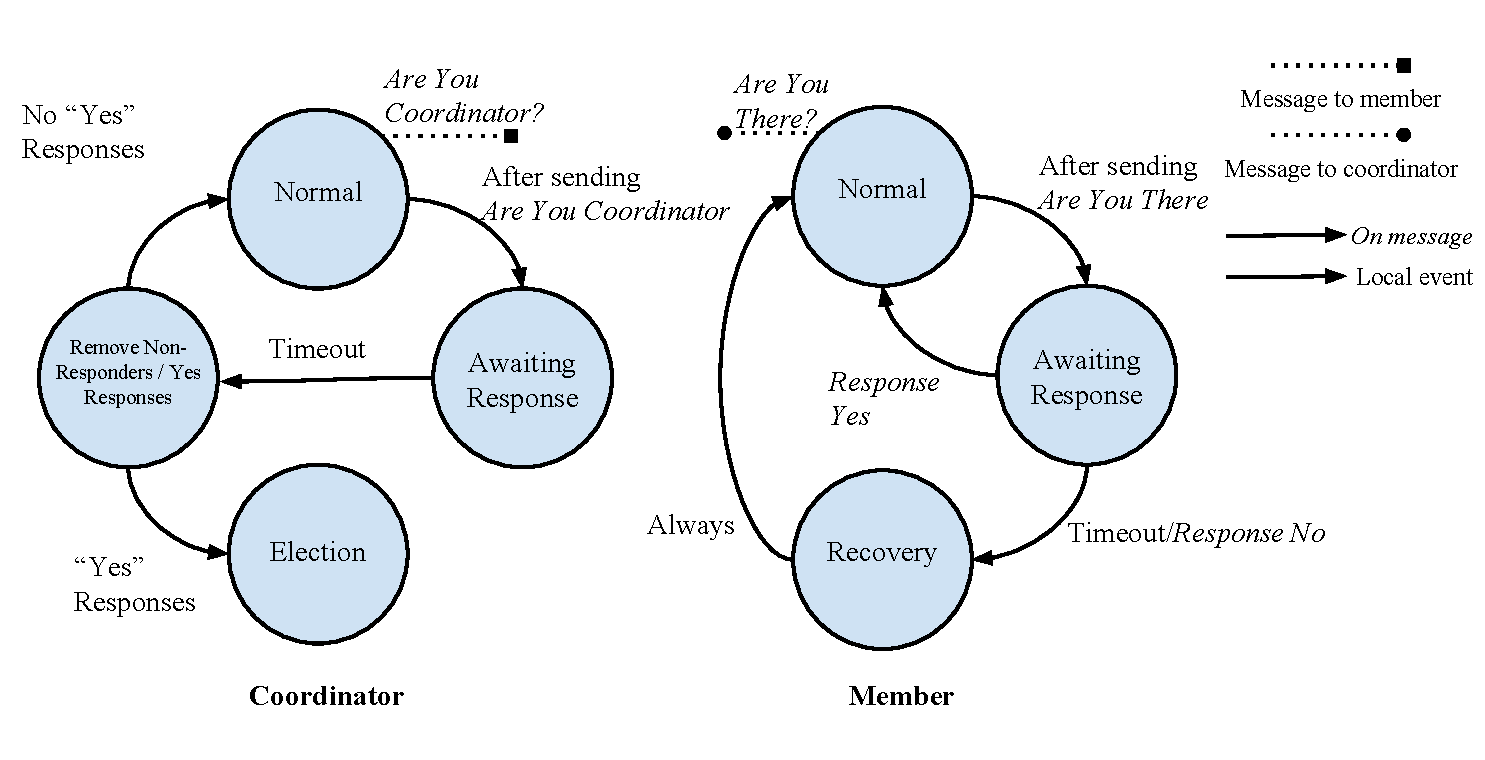
\includegraphics[width=\linewidth]{MaintainStateDiagram.pdf}
\caption[State machine for maintaining a group]{State machine for maintaining a group. The \ac{AYC} messages are the same as those in Figure \ref{fig:statemachine}. \ac{AYC} and \ac{AYT} are periodically sent by processes, and responses to those messages are immediately sent by the receiving process. In the modified algorithm, the member does not enter the recovery state if they do not receive an AYT response before the timeout expires.}
\label{fig:statemachine2}
\end{figure*}


\section{Model Construction}


\section{Highest Priority Process}

\subsection{State Determination}

% Show that the state of the group in the ready set of the orignal algorithm is an N set.
% Show that the members also have an N set.
In the Garcia-Molina version of the algorithm, processes distribute a list of processes that have accepted their invite.
Let $i$ be the coordinator of a group distributing ready messages.
The process $i$ has a list of processes that have accepted its invite.
Let $\varphi_x$ be a wff that indicates that some process $x$ is part of $i$'s group.
Let $R = \{ \varphi_x | x \in AcceptedInvite \} \cup \{ \varphi_i \}$ be the set of processes that have accepted $i$'s invite.
To finalize the group, $i$ will distribute $R$ to each process described in $R$.
If a processes does not receive $R$ it will not be in the group.

\begin{thm}
    In the original algorithm, each process is MSDND secure on $\varphi_x$ for each $x$ that is not $i$ or itself ($j$).
\end{thm}

\begin{proof}
\begin{case}
    The case where $x = i$ or $x = j$.
\end{case}

If we assume that the authenticity of messages is not questioned in this environment, a ready message from $i$ must mean $i$ is a part of the group.
Therefore, $i$'s inclusion in the group is MSDND insecure to $j$

If $j$ accepts the ready message, that process will be a part of the group in $R$ and since $j$ knows its own state, $j$ knows it is a part of $R$.

\begin{case}
    The case where $x \neq i$ and $x \neq j$
\end{case}

For process $i$, $i$ distributes $R$ to each other process in $R$.
Let $Q$ be some set of processes that do not receive the $R$ set.

\begin{table}[h!]
\centering
\small
\begin{tabularx}{\linewidth}{l X X}
1. & $I_{j,i} R \forall j \in R $ & $i$ distributes the list of processes that have accepted the invite.  \\
2. & $\neg(B_x I_{x,i} R \wedge T_{x,i} R) \forall x \in Q$ & Processes in $Q$ do not receive $R$. \\
3. & $B_x I_{x,i} R \wedge T_{x,i} R \forall x \not \in Q$ & Processes not in $Q$ receive $R$. \\
    4. & $w \not \vDash V_{B_x R}^{j}(w) \forall \{x | x \not \in \{i,j\}\}$ & $j$ does not know which processes received $R$ \\
\end{tabularx} \\~\\
Therefore, the receipt of $R$ by other members of the group is MSDND secure to $j$.
\label{tab:readynsetproof}
\end{table}
\end{proof}

\begin{cor}
    The set of processes in the ready message is an $N_i$ set, where $i$ the group's coordinator.
\end{cor}

Since every wff in $R$ is MSDND secure, $R$ must be an $N_i$ set, and consequently, $L_i = \emptyset$.
As a consequence, the group leader only has an estimate of the system, which may be an overestimate ($M_i \subseteq N_i$)

% Show that with the ready ack, the leader has an L set.
With an ready acknowledgment message from members of the group, the Leader can construct an $L_i$ set, which underestimates the state of the system.
From previous chapter, we have shown that with message passing and omission, at least one process is left insecure to the other.

\begin{thm}
    If a process $j$ sends a ready acknowledgment message to $i$, $j$'s inclusion in the $i$'s view of the system state is MSDND secure to $j$
\end{thm}

\begin{proof}
Proof: When $j$ sends the ready acknowledge message to $i$, it is uncertain if the acknowledgment message is actually delivered.
From Theorem \ref{case:generalsn0}, we know that $j$ is now MSDND insecure to $i$, but $i$ is insecure to $j$.
Using the ready acknowledgment messages, $i$ can then valuate $B_i B_j \varphi_j$ for every $j$ that sends an acknowledgment message.
\end{proof}

Once the ready acknowledgment messages have been sent to the leader, the group can begin to interact.
As it is impossible for the members of the group to be distributed the $L_i$ set, they must operate using the $N_i$ set they received from the coordinator.
Messages from other processes which could only have been sent if they are a part of the $M_i$ sent can leak to the receiving processes their receipt of the $R$ set from $i$.
For the purpose of model construction, the determination of members of $M_i$ that are not in $L_i$ may be undesirable for a \ac{DTMC} since it may involve changing the state captured for the chain at the incorrect moment.
Instead, for simplicity, while the leader can update their $L_i$ set with leaked information, we avoid doing so to preserve the memorylessness property in the following sections.
We defined the state of the system as the cardinality of the processes mentioned in the $L_i$ set.

% Show that inclusion in M but not L is leaked by AYC to ``member''

% Show that with a synchronized communication the priority of the leader can be determined.

\subsection{Memorylessness}

\begin{figure}[]
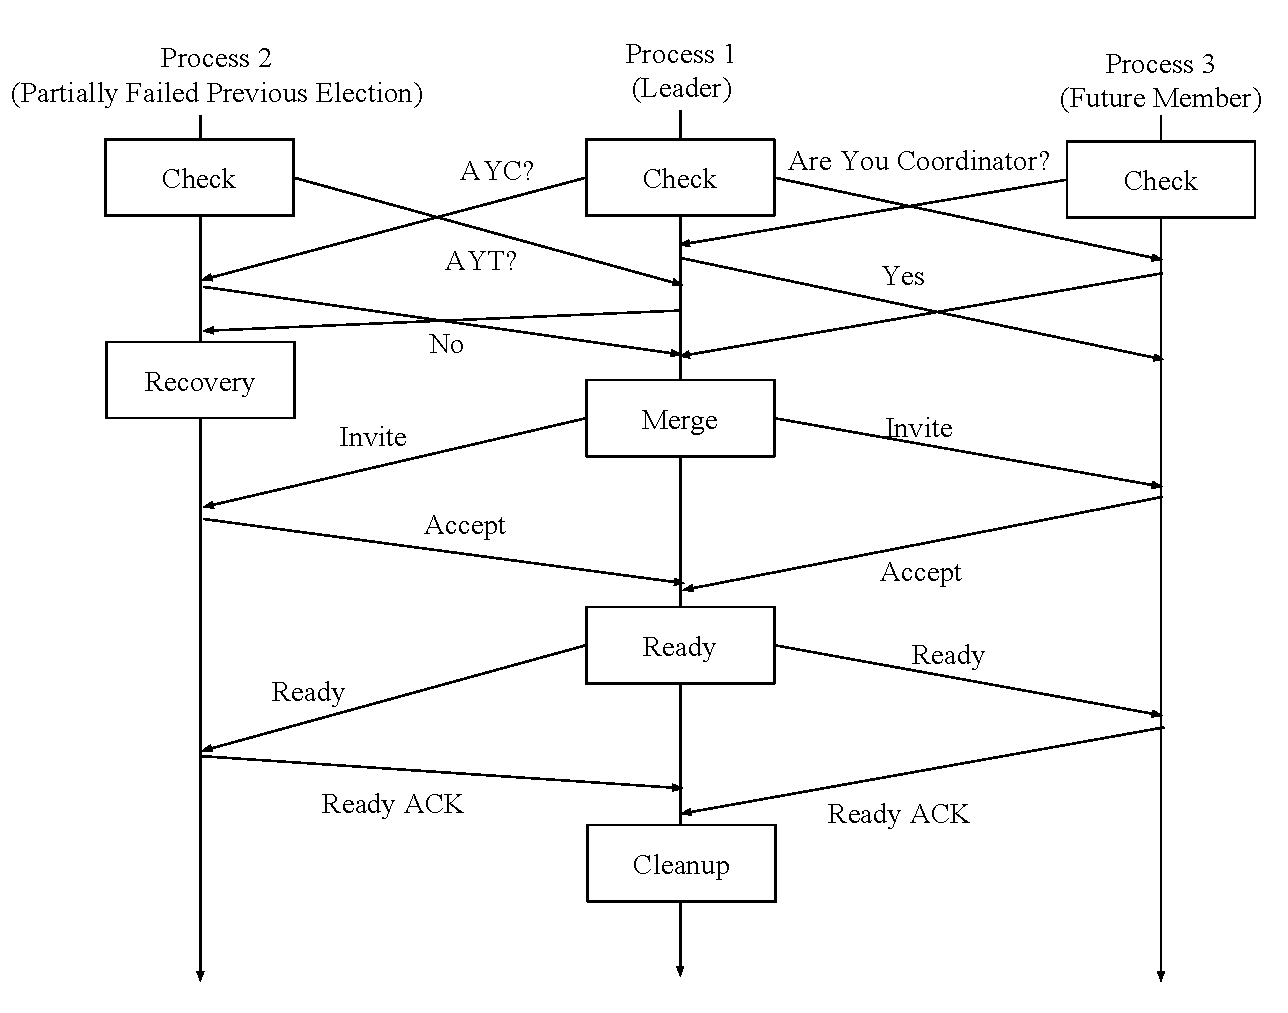
\includegraphics[width=\linewidth]{ElectionMessages}
\caption{Diagram of message exchanges for an election.}{Diagram of message exchanges for an election. In the figure, process 2 almost completed the previous election, and considers itself a part of process 1's group, but process 1 does not. Process 3 does not consider itself a part of process 1's group before the election begins. Both process 2 and process 3 need to successfully exchange the same number of messages to successfully complete the election.}
\label{fig:electionmessages}
\end{figure}

% Stage 1: AYC / AYT
% Show that maint. takes so many messages
% Show that leader discovery for election takes so many messages
% Show that a process in M but not L needs to many messages to do the above, which is equal.
The a process can update $L_i$ with leaked information.
To ensure the memorylessness property we are interested in capturing when a process receives the ready message, but the acknowledgment is lost, meaning the process is not included in the $L_i$ set.
We wish to ensure that the process can determine its own exclusion in $L_i$ so it can behave as though it is not in $M_i$.
To do this, we attach an additional field to the \ac{AYC} message to indicate if the coordinator $i$ considers the receiving process $j$ a part of the $L_i$ set.
This value obviously leaks to the receiving process that it is not part of $L_i$ and it should behave accordingly.

Likewise, for the coordinator, an \ac{AYT} message leaks to the coordinator that the sending process is a part of the $M_i$ set, if it is not in $L_i$.
Since the behavior of the process in $M_i$ is defined to behave as though it was not in $L_i$, the coordinator should do the same.
This should be the case even if the process sending \ac{AYT} has already responded negatively to an \ac{AYC} from $i$.
For the purpose of memorylessness, $i$ should consider $j$ to have responded in the affirmative.

% Stage 2:
% Show that the probability of an invite working is the probability of delivering an invite
% + all the lower priority invites not arriving
% Show that at this point M/L inclusion doesn't matter any more.
Processes determine which invite to accept based on the exchange of the \ac{AYC} messages.
Processes always seek to reach the ``lowest energy state'': they wish to be in a group led by the coordinator with the highest priority.
Since the process has determined which invite it will accept, the probability of receiving that invite is the probability that process did not interact with a higher priority process that caused it to expect an invite.
Processes will submit AYC messages to higher priority processes that are not its coordinator, even if they are in a group.
As a result, the processes will always seek highest priority, regardless of their current group.
More importantly, this releases the process from obligations on its next state from the state of other processes in the system.

% Stage 3:
% Show that ready only depends on the sucessful delivery of ready
% & Ready ack.
A process will only accept an invite if it receives it and it has determined it is the invite it wishes to accept.
This result allows a process to determine the likelihood of an invite being accepted.
This probability is based on the probability the higher priority process selecting that process to send invites to, and the lower priority process selecting that invite.

In Figure \ref{fig:electionmessages}, we diagram the sequence of message exchanges and function calls for two possible states a process that is not in the leader's group.
In the first state, the process nearly completed an election the previous round, but the read acknowledgement message was not delivered in time, resulting in the process being in the $M_i$ set.
In the second state, the process is not in the leader's group.
As shown in Figure \ref{fig:electionmessages}, both cases require the same number of messages to be delivered for the process to be considered a part of the group.

\subsection{Model Construction}

Based on the state determination and memorylessness arguments presented, the highest priority process operates independent of the state of the other processes in the system.
The highest priority processes invites are always accepted, and the structure of the algorithm prevents any process from being locked out of participating in a round of execution based on the outcome of the previous round.
Therefore, for every observation of the system state the highest priority process makes, the next round of execution for all the other processes favors the high priority process, ensuring that its observation corresponds directly with the system state.

In each round, the behavior is described by two components: maintaining a group and inviting other processes into the group.
The coordinator will exchange an ``Are You Coordinator'' message and the peer will respond to verify is still available.
To maintain a group of $m$ other processes, the probability is defined as a random variable with the following \ac{pdf}:

\begin{equation}
 \Pr_{M}(X=k; m) =
   \begin{cases}
    \binom{m}{k} p^{2k}(1-p^2)^{m-k}, & \text{if } 0 \leq k \leq m \\
    0,                                & \text{otherwise} \\
  \end{cases}
\end{equation}

Where $k$ is the number of processes remaining in a group selected from $m$ processes.
A process will leave a group if, from the considered process's perspective, they do not respond to an ``Are You Coordinator'' message.

To invite other processes to the group, the two processes ultimately exchange up to 8 messages.
In a round, a single process can invite many other processes to its group.
From a selection of $n$ other coordinators, the probability distribution for joining a new group with $k$ of the $n$ processes is:

\begin{equation}
    \Pr_{I}(Y=k; n) =
    \begin{cases}
        \binom{n}{k} p^{8k}(1-p^8)^{n-k}, & \text{if } 0 \leq k \leq n \\
        0,                                & \text{otherwise} \\
    \end{cases}
\end{equation}

In the profile chain, in a state $s$ that describes the number of processes in a group, the probability of transitioning from $s$ to $s'$ with $n$ total processes (including the considered process) is:

\begin{align} \Pr_{T}(Z=s'; n; s) = \sum_{i=0}^{s-1} &\Pr_{M}(X=i; s-1) \cdot
\nonumber \\ &\Pr_{I}(X=s'-i; n-s-1) \end{align}

From this distribution, a set of transition probabilities can be calculated for a given omission rate $p$ and number of processes $n$.
This set of transition probabilities forms a profile Markov chain $P$, which can be evaluated to for any number of processes $n$ and omission rate $p$.
The generated profile chain is ergodic when $0<p<1.0$. The profile chain is a stationary Markov chain.

\subsection{Model Validation}

%State that verification of the profile chain via statistical tests is important. State that if P and T are ergodic stochastic sources and can generate similar sequences if they have the same transition probabilities. State that statistical tests can identify if two chains are different at some significant level.

To assert the closed form profile chain accurately represents the implementation of the algorithm, it must be validated.
Since $T$ and $P$ are ergodic, they can be checked for equivalence using a goodness-of-fit test.
If the goodness-of-fit test indicates the chains are equivalent, they will generate similar sequences and have similar properties when analyzed.
Therefore, generated $P$ chains can be used to analyze the behavior of the algorithm during live execution with changing conditions.

To verify the test chain $T$ is equivalent to the profile chain $P$, a $\chi^2$ goodness-of-fit test is employed.
The null-hypothesis of this test ($H_{0}$) asserts the profile chain $P$ is equivalent to the test chain $T$:

\begin{equation} H_{0}: T = P \end{equation}

With an alternative hypothesis that the two chains are not equivalent:

\begin{equation} H_{1}: T \neq P \end{equation}

The $\chi^2$ test measures the goodness-of-fit for a complete chain by combining the measurements of goodness of fit for the transitions away from each state.
Therefore, the goodness of fit test for the chain is a summation of tests for each state:\cite{MARKOV3}

\begin{equation} \chi^2 = \sum_{i}^{m} \sum_{j}^{m} = \frac{n_{i}(P_{ij}-T_{ij})^2}{P_{ij}} \end{equation}

Where $n_{i}$ is the number of times the state $i$ was observed in the input sequence used to construct the test chain $T$.
The summation is distributed as $\chi^2$ with $m(m-1)$ \ac{DF} if all entries in $P_{ij}$ are non-zero.
In this work, all transitions in the profile Markov chain $P$ are non-zero when $0<p<1.0$.
However, the probability of some transitions may be extremely small.
The $\chi^2$ value was compared to a \ac{CV} giving a measure of how likely it was $H_{0}$ could not be rejected.
This work selected an $\alpha = 0.05$ significance level to reject the hypothesis $T=P$.

If the hypothesis $H_{0}$ were to be rejected, it would indicate the test chain and profile chain differ significantly.
As a consequence of rejecting the hypothesis, the implementation would have behavior from the generated closed form solution.

To verify the model, it was compared to runs of an implementation of the algorithm.
Test data was collected for systems with 3, 4, 5 and 6 processes.
Information was collected from sufficiently long runs of the system with an omission rates between 0.05 and 0.95 tested at intervals of 0.05.
Table \ref{tab:chisummary} shows the measured error and p-value for the worst observed error for each number of processes.
Since the measured error is less than the critical value and the p-value is greater than 0.05, we cannot reject $H_0$. 
As a consequence, the profile chains ($P$) are representative of the behavior of the algorithm's implementation.

\begin{table*}[!t]
\centering
\begin{tabular}{ c | c c c c c}
  \hline
  Processes & DF & CV & Worst Error & $\Pr(WorstError)$ &  p-value \\ \hline
  3 & 6 & 12.6 & 8.90 & 0.80 & 0.18 \\
  4 & 12 & 21.0 & 14.55 & 0.75 & 0.27 \\
  5 & 20 & 31.4 & 23.47 & 0.65 & 0.27 \\
  6 & 30 & 43.8 & 32.69 & 0.85 & 0.34 \\
\end{tabular}
\caption{Summary of $\chi^2$ tests performed.}
\label{tab:chisummary}
\end{table*}

\section{Profile Chain Analysis}

Resources can only be managed effectively when multiple \ac{DGI} coordinate together to manage those resources.
Without another DGI to coordinate with, the DGI has a limited range of options to manage power generation, storage and loads.
Therefore, the amount of time DGI will spend coordinating with another process is of particular interest.
\cite{CRITIS2012} defines an \ac{IGT} metric to measure the amount of time a DGI process spends coordinating with at least one other process.
In this work, we define \ac{IGT} based on the steady state of the profile chain.
Let $\pi=Steady(P)$ for some profile chain.
The \ac{IGT} is the sum of all states in $\pi$, save the first state where the process is alone:

\begin{equation} IGT = \sum_{i=2}^{m} \pi_i \end{equation}

The \ac{IGT} is a number between 0 and 1.
It represents the probability a random observation sees a group of at least two members.
The steady state distributions are presented as stacked bar graphs in Figures \ref{fig:ss-3process}, \ref{fig:ss-4process}, \ref{fig:ss-5process} and \ref{fig:ss-6process}.
Each complete bar in the graph indicates the \ac{IGT}.
Additionally, Figures \ref{fig:ss-3process}, \ref{fig:ss-4process}, \ref{fig:ss-5process} and \ref{fig:ss-6process} also contain the average group size (AGS), when the system has reached the steady-state, plotted as a fraction of the total number of processes.
Let $P$ be the steady-state distribution vector for some number of processes, $n$, and a given omission rate:

\begin{equation} y = \frac{\sum_{i=1}^{n} P_{i}*i}{n} \label{eq:ss-means} \end{equation}

where $y$ is the plotted \ac{AGS} as a fraction.

The components of each bar represent the probability the system is in a specific state for a random observation of the system.
The height of the component represents the relative probability of observing that state when in a group.

\begin{figure}
    \centering
    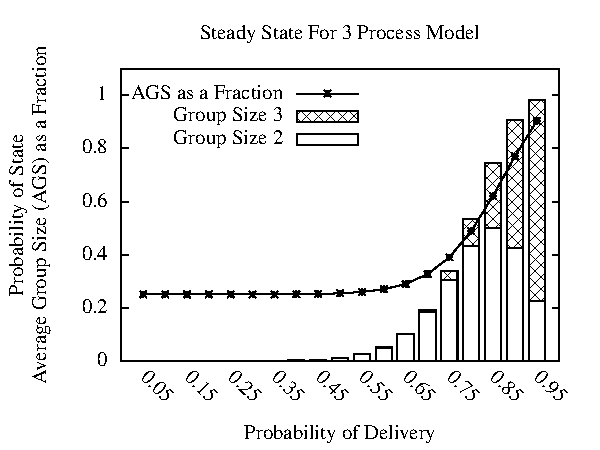
\includegraphics[width=0.6\linewidth]{ss-3process.pdf}
    \caption{Steady state distribution for 3 processes as well as the \ac{AGS} as a fraction of total processes.}
    \label{fig:ss-3process}
\end{figure}

\begin{figure}
    \centering
    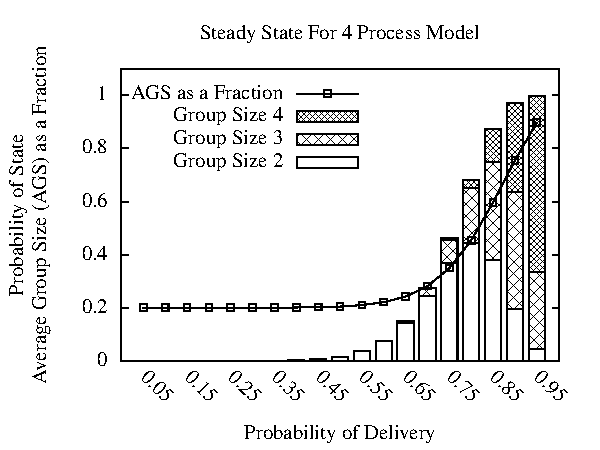
\includegraphics[width=0.6\linewidth]{ss-4process.pdf}
    \caption{Steady state distribution for 4 processes as well as the \ac{AGS} as a fraction of total processes.}
    \label{fig:ss-4process}
\end{figure}

\begin{figure}
    \centering
    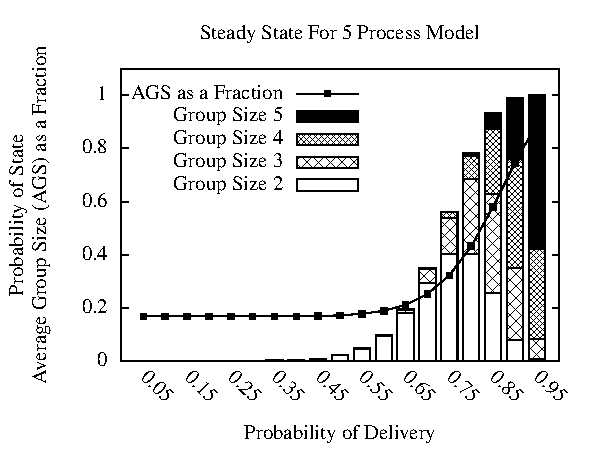
\includegraphics[width=0.6\linewidth]{ss-5process.pdf}
    \caption{Steady state distribution for 5 processes as well as the \ac{AGS} as a fraction of total processes.}
    \label{fig:ss-5process}
\end{figure}

\begin{figure}
    \centering
    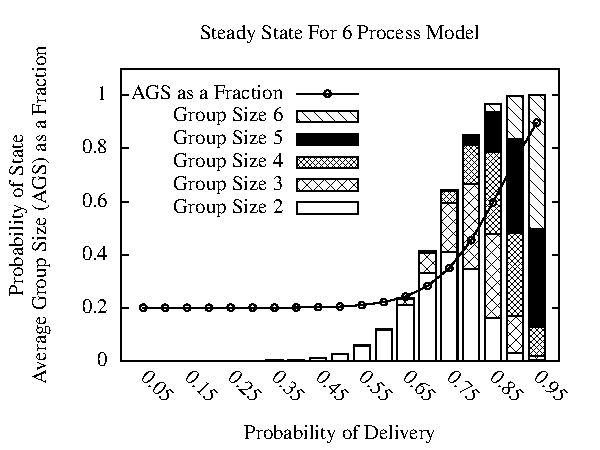
\includegraphics[width=0.6\linewidth]{ss-6process.pdf}
    \caption{Steady state distribution for 6 processes as well as the \ac{AGS} as a fraction of total processes.}
    \label{fig:ss-6process}
\end{figure}

The profile chain can be used to ensure the \ac{FREEDM} smart grid is able to continue operating despite network issues.
The profile chain can be combined with different message sending strategies to maintain service.
For example, the DGI can change to a slower mode of operation to ensure operation continues normally despite connectivity issues.
By selecting different strategies depending on the message delivery probability the DGI can offer high performance in good network conditions and an acceptable level of service during faults.
The profile chain can be extended to an arbitrary number of processes as shown in Figure \ref{fig:ss-means}.
In Figure \ref{fig:ss-means}, the steady-state of the system is used to compute a weighted average of the group size.
To compare the produced steady states, the weighted average was plotted as a percentage of all processes in the system.
Values in Figure \ref{fig:ss-means}, were plotted using Equation \ref{eq:ss-means}.
Therefore, Figure \ref{fig:ss-means}, shows the average percentage of total processes that will be in the group in a steady-state system.

\begin{figure}
    \centering
    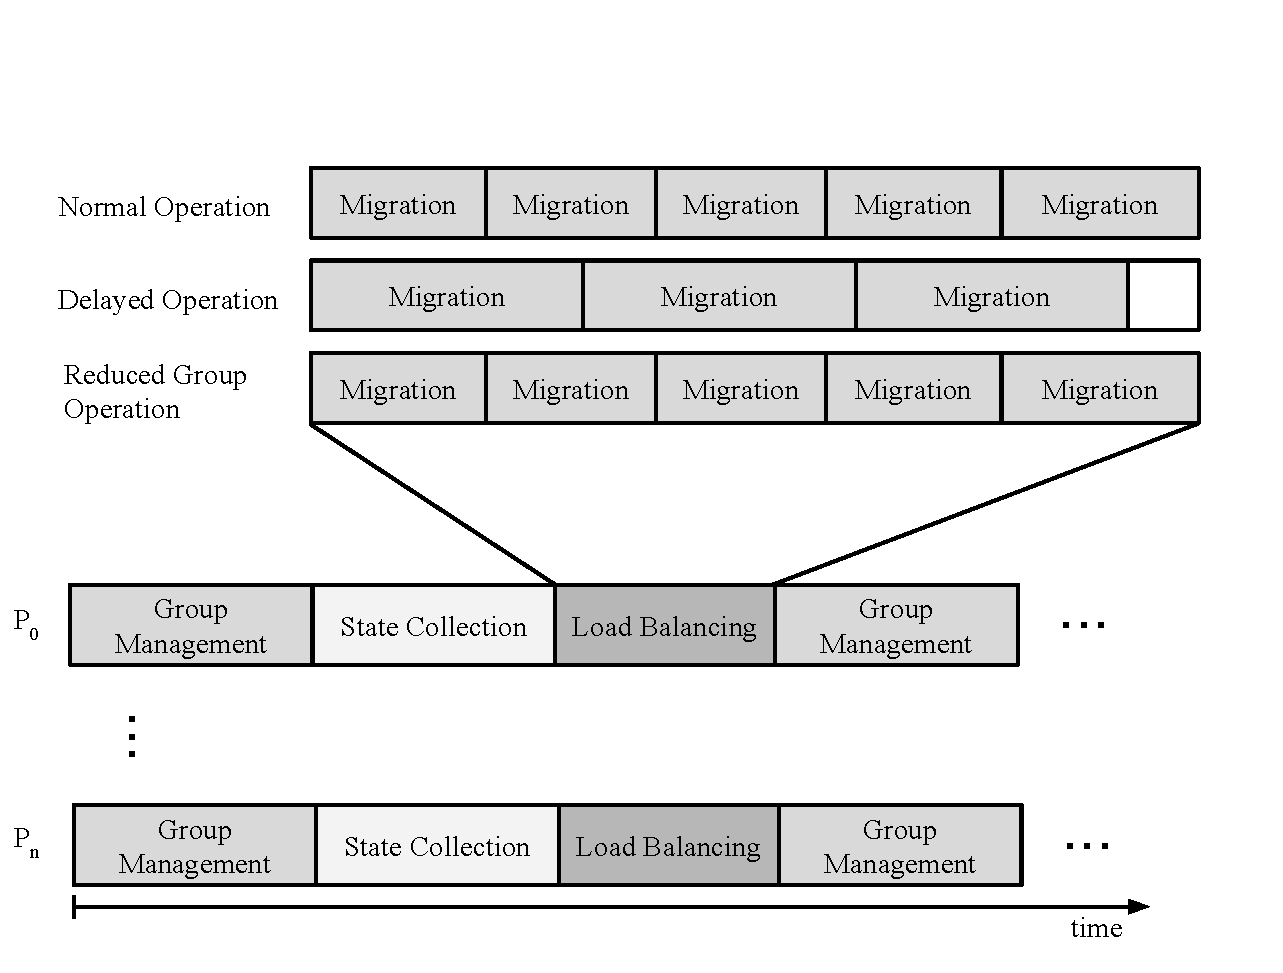
\includegraphics[width=0.75\linewidth]{schedule.pdf}
    \caption[Example DGI schedule]{Example DGI schedule. Normal operation accounts for a fixed number of migrations each time the load balancing module runs. Message delays reduce the number of migrations that can be completed each round. However, reducing the group size allows more migrations to be completed (because fewer messages are being exchanged) at the cost of flexibility for how those migrations are completed.}
    \label{fig:schedule}
\end{figure}

The DGI employed a round-robin schedule where each module is given a predetermined amount of time to execute.
This schedule was determined by the number of DGI that could be grouped together and the expected cyber network conditions.
Additionally, the Load Balance module, which managed the power resources was scheduled to run multiple times in a long block before the group was evaluated for failure.
This schedule is depicted in \ref{fig:schedule}.
The system began by using group management to organize groups.
Next load balancing ran to manage power resources in the created group.
Finally, state collection collected a casually consistent state to be used for reporting and offline analysis.
If message delays occurred, the number of migrations load balancing could perform was reduced.
However, by reducing the group size, the number of messages sent by load balancing could be reduced, allowing for a greater amount of work to be done.
The outcome of an election had a direct effect on how effectively the DGI can manage resources.
Therefore the steady-state analysis gives a good indication of how well the DGI could manage those resources in the future.
%Interestingly, the average group size as percentage of the total processes seems to be converging asymptotically, to a fixed value for each plotted probability as the number of processes increases.

\begin{figure}
    \centering
    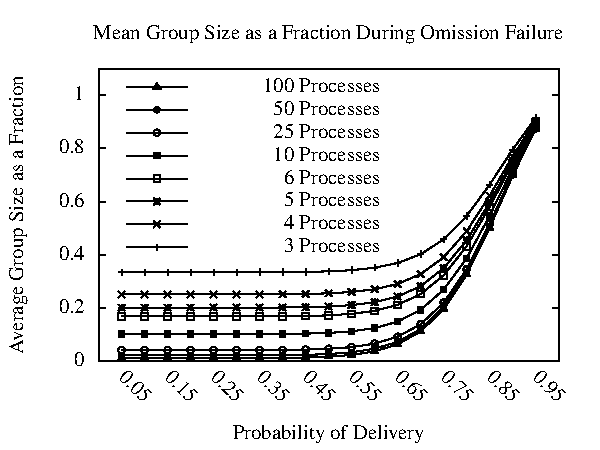
\includegraphics[width=0.6\linewidth]{ss-means.pdf}
    \caption{Average group size as a percentage of all processes in the system for larger systems.}
    \label{fig:ss-means}
\end{figure}

This information can also be used to anticipate faults and mitigate them before they occur.
Modern routers can supply an expected congestion notification as part of the IP header\cite{ECN2}.
When congestion is anticipated, the coordinator can preemptively split the group to reduce congestion.
This is possible because the algorithm's message complexity is $O(n^2)$.
Future work will combine this analysis with \ac{ECN} techniques to preemptively change the behavior of DGI to ensure a good level of service.
If dropped messages account for an omission rate of even 0.15 from future congestion, performing a coordinated group division can potentially save several rounds of transient states.
Breaking the large groups into smaller sets can drastically reduce the number of messages transmitted and help relieve congestion.
Additionally, the coordinator can design the split to ensure work can continue when the groups are split, by mixing supply and demand processes.
The division can also account for the placement of congested routers for targeted congestion relief.
Furthermore, since the required execution time is a function of group size, the DGI can use the additional execution time within the same real time schedule to use more reliable techniques to deliver messages.


In Figure \ref{fig:schedule}, Group Management's execution is broken into four steps: check, merge, ready, and cleanup.
Between each step, the DGI waits while messages and their replies are delivered.
The leader election algorithm expects that all replies arrive before the next step of the algorithm is executed.
If a message does not arrive during the wait period, before the next step of execution the message is considered lost.
If it arrives later, it is ignored by the algorithm.
While dynamically adjusting the synchronized schedule is not feasible during failure, adjusting the number of messages sent (by sending fewer "Are You Coordinator" messages, for example) is.
By sending fewer messages, the number of packets in the communication network is reduced, and the savings in processing can allow multiple delivery attempts in the scheduled wait time.

\section{Lower Priority Process}

A model cannot be constructed for a process that is not the highest priority for this algorithm.
The lower priority process cannot know which processes are already in a group with the higher priority process.
In the execution model we have presented, the inclusion of a process in a higher priority process's group is MSDND secure.
There is no way to for a process that is not in a group to know what processes are in any group except its own.

% For a lower priority process, the probability that an invite will work depends on the probability that that process is
% Not already in a higher priority group IE, it depends on the outcome of the last election & staying in a group this time
% For the highest priority process, it doesn't matter what the outcome of the last election was, it can merge that process into its group.
% So we can demonstrate 2 things: First, the probability of inviting a process from a lower priority process would violate the memorylessness property
% And secondly, the state of the other process being in the group is MSDND secure
% A result is secure until it is revealed and then when the process changes variables it is secure again.
%TODO...

% Set of worlds may need to be defined over a round of execution? Keep space smaller, fixes belief revision.
% You can show two worlds, one where the process is group and the other where its ungrouped have different outcomes
% for a third process.

% You can show that the there is no way for the process to know that, the state is MSDND secure.
% Lastly, we need to show there is no way of making it independent
% There's several different versions for this:
% It may be sufficent to show that it can only be memoryless for the leader, because only the highest priority
% can know that the invites will work, every other process depends on the state of the highest priority process
% which is not memoryless. No matter how it is defined, allowing a process with a higher priority to determine
% The state prevents a lower priority one from doing so.

% Really, the arguement is, if the state affects you can you can't determine it, you can't construct a model.
% Maybe as a corrollary?
% Well, in this case, the highest priority process is not affected by the state it doesn't know.
% Can I prove that if the markov chain is first order, some other process must always be affected by the hidden state?

\section{Independent Algorithm}

If we restrict the algorithm to be more like the Bully algorithm, running the partially synchronous environment, any process can construct their model.
This is accomplished by removing the maintenance portion, releasing each process from the previous state of execution entirely.
% Interesting... can I prove that if any process depends on a previous state, no other process can be memoryless?

% Send an invite to each lower priority process. (Each receives n invites)
% Each process collects all the invites and selects the highest priority
% Send response to highest priority.
% Process sends ready to recipients
% recips send ready ack

% probability of success = probability higher priority's invites don't arrive.
% * the probability the response makes it
% * the probability the ready makes it
% * the probability the ready ack makes it


